\chapter{Pareto family}
%%%%%%%%%%%%%%%%%%%%%%%%%%%%%%%%%%%%%%%%%%%%%
\section{Pareto distribution}
name??
\subsection{Characterization}
\begin{wrapfigure}{r}{0.5\textwidth}
  \vspace{-20pt}
  \begin{center}
    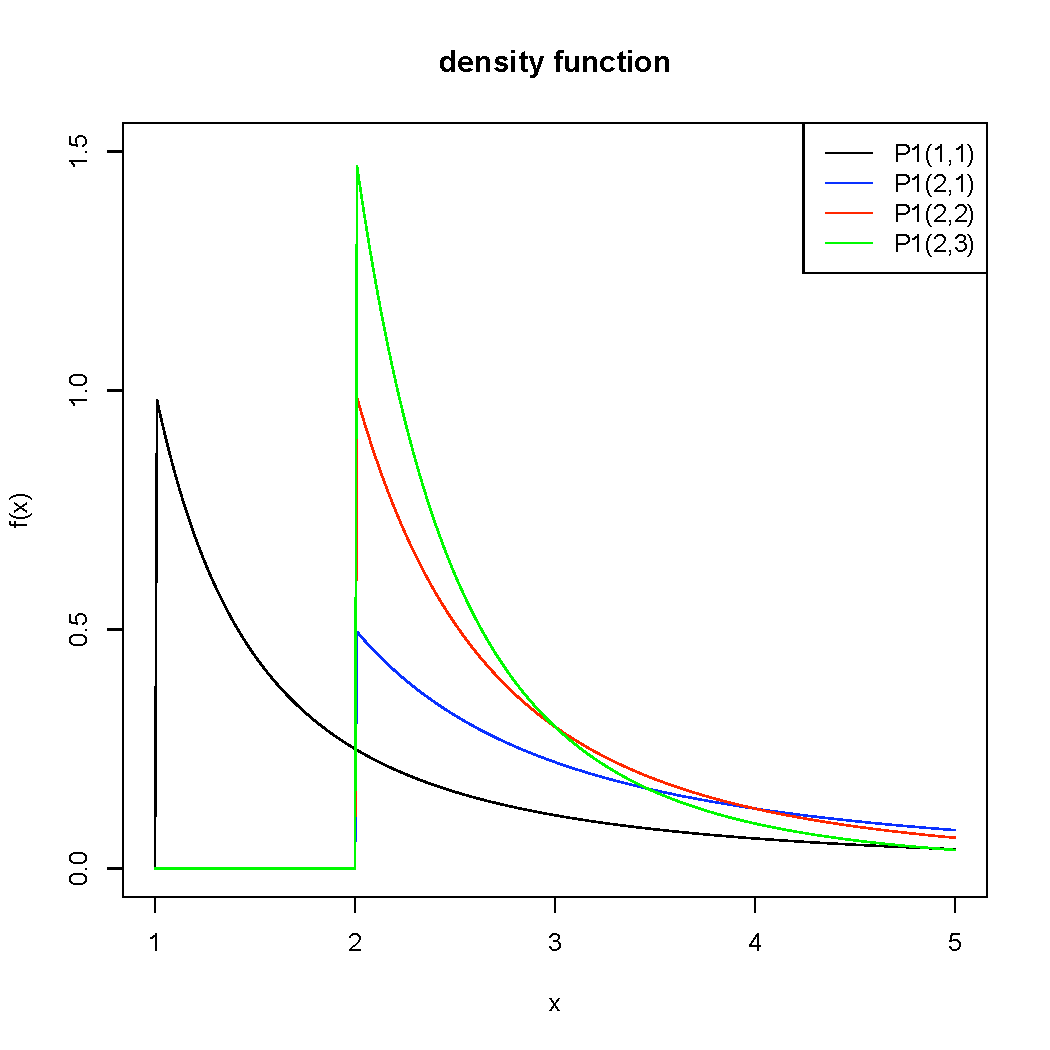
\includegraphics[width=0.48\textwidth]{img/pareto1zoom}
  \end{center}
  \vspace{-20pt}  
  \caption{Density function for Pareto I distributions}
  \vspace{-20pt}  
\end{wrapfigure}
The Pareto is widely used by statistician across the world, but many parametrizations of the Pareto distribution are used. Typically two different generalized Pareto distribution are used in extrem value theory with the work of Pickands et al. and in loss models by Klugman et al. To have a clear view on Pareto distributions, we use the work of \cite{arnold83}.
Most of the time, Pareto distributions are defined in terms of their survival function $\bar F$, thus we omit the distribution function. In the following, we will define Pareto type I, II, III and IV plus the Pareto-Feller distributions. 

\subsubsection{Pareto I}
The Pareto type I distribution $\mcal Pa_I(\sigma, \alpha)$ is defined by the following survival function
$$
\bar F(x) = \left(\frac{x}{\sigma}\right)^{-\alpha},
$$
where $x>\sigma$ and $\alpha>0$. Therefore, its density is 
$$
f(x) = \frac{\alpha}{\sigma} \left(\frac{x}{\sigma}\right)^{-\alpha-1},
$$
still for $x>\sigma$. $\alpha$ is the positive slope parameter\footnote{the slope of the Pareto chart $\log \bar F(x)$ vs. $\log x$, controlling the shape of the distribution.} (sometimes called the Pareto's index) and $\sigma$ is the scale parameter.
Pareto type I distribution is sometimes called the classical Pareto distribution or the European Pareto distribution.

\subsubsection{Pareto II}
\begin{wrapfigure}{r}{0.5\textwidth}
  \vspace{-40pt}
  \begin{center}
    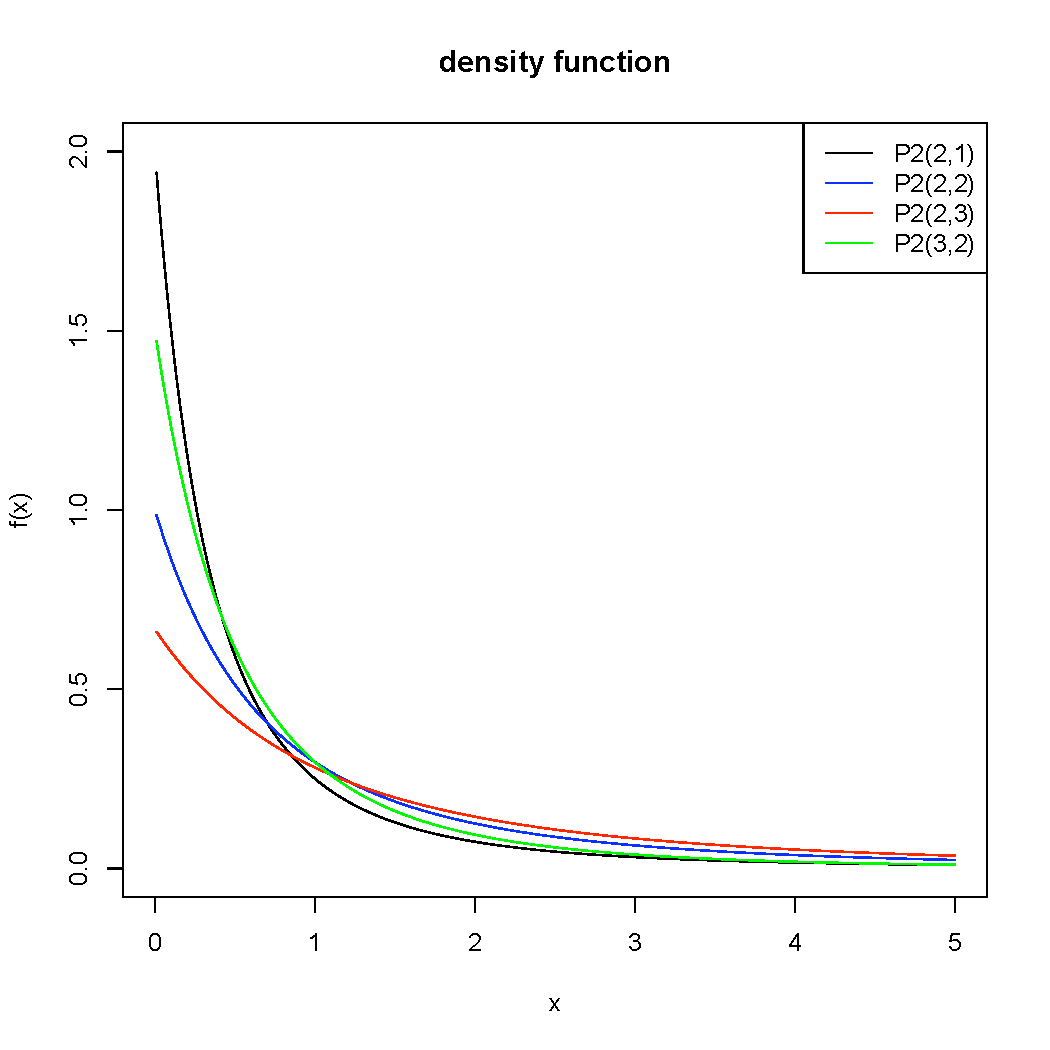
\includegraphics[width=0.48\textwidth]{img/pareto2zoom}
  \end{center}
  \vspace{-20pt}  
  \caption{Density function for Pareto II distributions}
  \vspace{-20pt}  
\end{wrapfigure}
The Pareto type II distribution $\mcal Pa_{II}(\mu, \sigma, \alpha)$ is characterized by this survival function
$$
\bar F(x) = \left(1+\frac{x-\mu}{\sigma}\right)^{-\alpha},
$$
where $x>\mu$ and $\sigma,\alpha>0$. Again $\alpha$ is the shape parameter, while $\mu$ is the location parameter. We can derive the density from this definition:
$$
f(x)= \frac{\alpha}{\sigma}  \left(1+\frac{x-\mu}{\sigma}\right)^{-\alpha-1},
$$
for $x>\mu$. We retrieve the Pareto I distribution with $\mu=\sigma$, i.e. if $X$ follows a Pareto I distribution then $\mu-\sigma+X$ follows a Pareto II distribution. The Pareto II is sometimes called the American Pareto distribution.

\subsubsection{Pareto III}
\begin{wrapfigure}{r}{0.5\textwidth}
  \vspace{-20pt}
  \begin{center}
    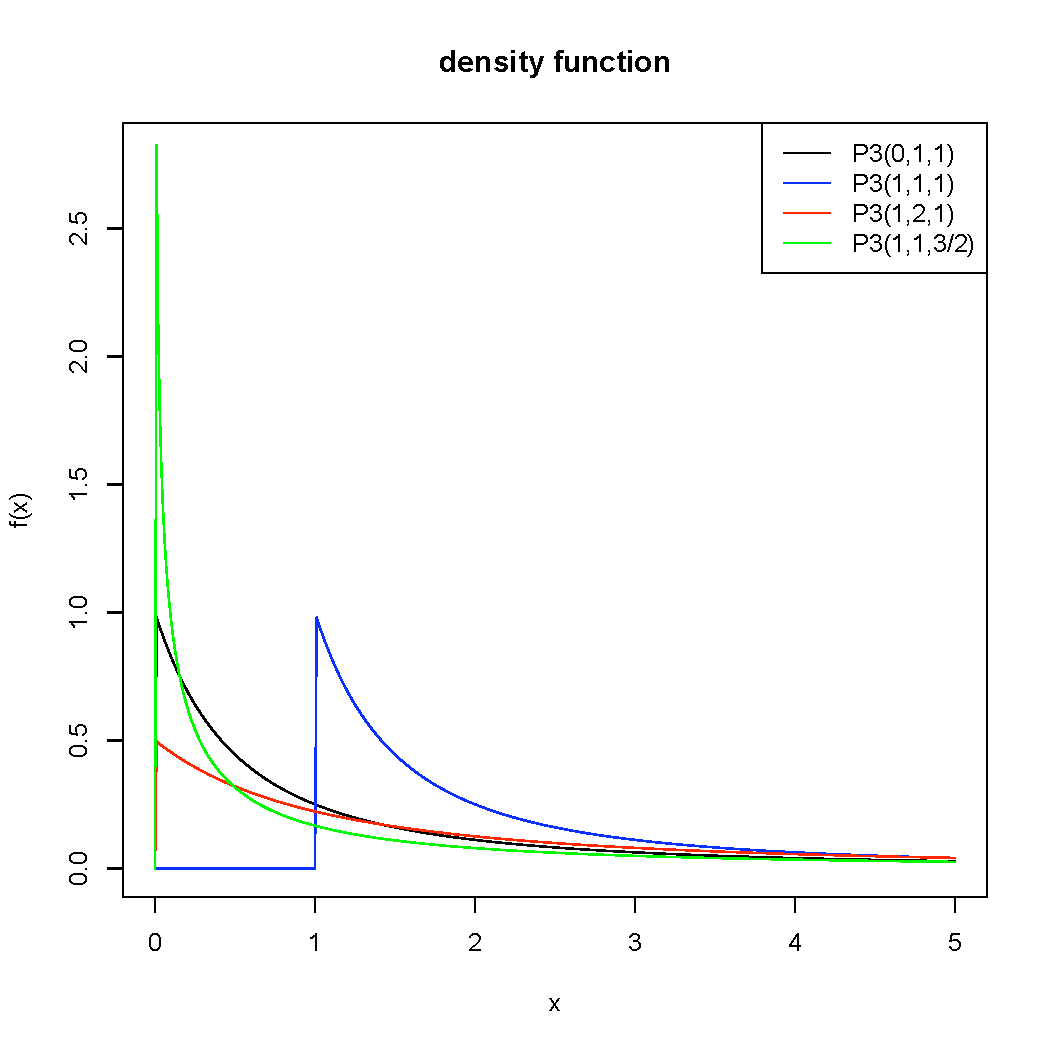
\includegraphics[width=0.48\textwidth]{img/pareto3zoom}
  \end{center}
  \vspace{-20pt}  
  \caption{Density function for Pareto III distributions}
  \vspace{-20pt}  
\end{wrapfigure}
A similar distribution to the type II distribution is the Pareto type III $\mcal Pa_{III}(\mu, \sigma, \gamma)$ distribution defined as
$$
\bar F(x)  = \left(1+\left(\frac{x-\mu}{\sigma}\right)^{\frac{1}{\gamma}}\right)^{-1},
$$
where $x>\mu$, $\gamma,\sigma>0$. The $\gamma$ parameter is called the index of inequality, and in the special case of $\mu=0$, it is the Gini index of inequality. The density function is given by
$$
f(x)  = \frac{1}{\gamma\sigma} \left(\frac{x-\mu}{\sigma}\right)^{\frac{1}{\gamma}-1} \left(1+\left(\frac{x-\mu}{\sigma}\right)^{\frac{1}{\gamma}}\right)^{-2},
$$
where $x>\mu$. The Pareto III is not a generalisation of the Pareto II distribution, but from these two distribution we can derive more general models. It can be seen as the following transformation $\mu+\sigma Z^\gamma$, where $Z$ is a Pareto II $\mcal Pa_{II}(0, 1, 1)$.

\subsubsection{Pareto IV}
\begin{wrapfigure}{r}{0.5\textwidth}
  \vspace{-20pt}
  \begin{center}
    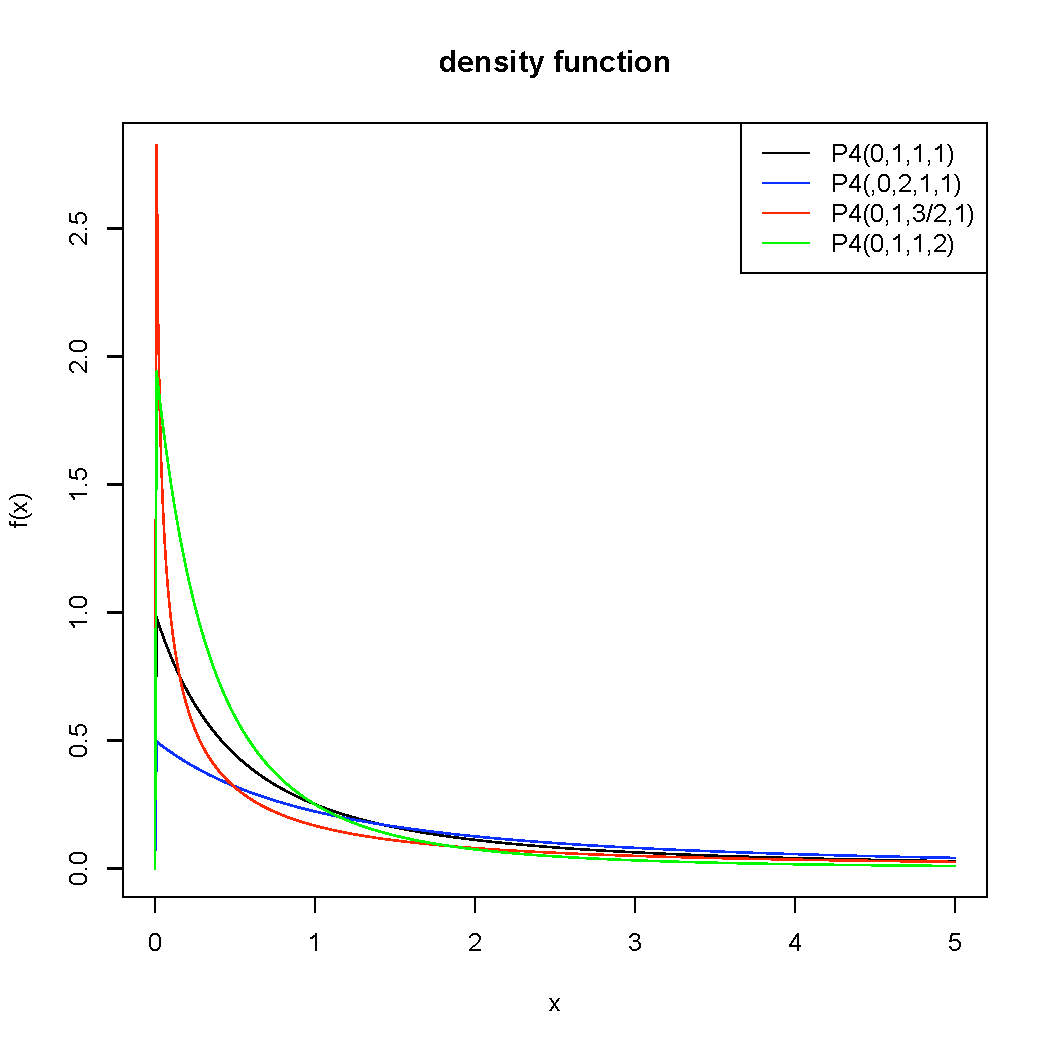
\includegraphics[width=0.48\textwidth]{img/pareto4zoom}
  \end{center}
  \vspace{-20pt}  
  \caption{Density function for Pareto IV distributions}
  \vspace{-20pt}  
\end{wrapfigure}
The Pareto type IV $\mcal Pa_{IV}(\mu, \sigma, \gamma, \alpha)$ distribution is defined by
$$
\bar F(x)  = \left(1+\left(\frac{x-\mu}{\sigma}\right)^{\frac{1}{\gamma}}\right)^{-\alpha},
$$
where $x>\mu$ and $\alpha,\sigma, \gamma>0$. The associated density function is expressed as follows
$$
f(x) = \frac{\alpha}{\gamma\sigma} \left(\frac{x-\mu}{\sigma}\right)^{\frac{1}{\gamma}-1} \left(1+\left(\frac{x-\mu}{\sigma}\right)^{\frac{1}{\gamma}}\right)^{-\alpha-1}
$$
for $x>\mu$.

Quantile functions for Pareto distributions are listed in sub-section random generation.

The generalized Pareto used in extreme value theory due to \cite{pickands} has a limiting distribution with Pareto II $\mcal Pa_{II}(0, \sigma, \alpha)$, see chapter on EVT for details. Finally, the Feller-Pareto is a generalisation of the Pareto IV distribution, cf. next section.

\subsection{Properties}

\subsubsection{Equivalence}
It is easy to verify that if $X$ follows a Pareto I distribution $\mcal Pa_I(\sigma, \alpha)$, then $\log X$ follows a translated exponential distribution $\mcal T\mcal E(\sigma, \alpha ?)$.

The Pareto type III distribution is sometimes called the log-logistic distribution, since if $X$ has a logistic distribution then $e^X$ has a Pareto type III distribution with $\mu=0$.

\subsubsection{Moments}
Moments for the Pareto I distribution are given by 
$E(X) = \frac{\alpha \sigma}{\alpha-1}$ if $\alpha > 1$, $Var(X) = \frac{\alpha \sigma^2}{(\alpha-1)^2(\alpha-2)}$ and $E(X^\tau) = \tau \frac{\alpha}{\alpha-\tau}$ for $\alpha >\tau$ and $\sigma=1$.

Moments for the Pareto II, III can be derived from those of Pareto IV distribution, which are
$$
E(X^\tau) = \sigma^\tau \frac{\Gamma(1+\tau\gamma)\Gamma(\alpha-\tau\gamma)}{\Gamma(\alpha)},
$$
with $-1<\tau\gamma<\alpha$ and $\mu=0$.

\subsubsection{Convolution and sum}
The convolution (i.e. sum) of Pareto I distributions does not have any particular form but the product of Pareto I distributions does have a analytical form. 

If we consider of $n$ i.i.d. Pareto I $\mcal Pa_I(\sigma, \alpha)$ random variables, then the product $\Pi$ has the following density
$$
f_\Pi(x) = \frac{\alpha \left(\sigma \log(\frac{x-\sigma}{\sigma}) \right)^{n-1} \left(\frac{x}{\sigma}\right)^{-\alpha}  }{x \Gamma(n)},
$$
where $x>\sigma$.

If we consider only independent Pareto I distribution $\mcal Pa_I(\sigma_i, \alpha_i)$, then we have for the density of the product
$$
f_\Pi(x) = \sum_{i=1}^n\frac{\alpha_i}{\sigma} \left(\frac{x}{\sigma}\right)^{-\alpha_i-1} \prod_{k\neq i}\frac{\alpha_k}{\alpha_i-\alpha_k},
$$
where $x> \prod_{i=1}^n\sigma_i$.

Other Pareto distributions??



\subsubsection{Order statistics}
Let $(X_i)_i$ be a sample of Pareto distributions. We denote by $(X_{i:n})_i$ the associated order statistics, i.e. $X_{1:n}$ is the minimum and $X_{n:n}$ the maximum.

For Pareto I distribution, the $i$th order statistic has the following survival function
$$
\bar F_{X_{i:n}}(x) = \sum_{j=1}^i \left(1+\frac{x}{\sigma}\right)^{-\alpha(n-j+1)} \prod_{\stackrel{l=1}{l\neq i}}^{i}\frac{n-l+1}{l-j},
$$
where $x>0$. Furthermore moments are given by
$$
E(X_{i:n}^\tau) = \sigma^\tau \frac{n!}{(n-i)!} \frac{\Gamma(n-i+1-\tau\alpha^{-1})}{\Gamma(n+1-\tau\alpha^{-1})},
$$
for $\tau\in\mbb R$.

For Pareto II distribution, we get
$$
\bar F_{X_{i:n}}(x) = \sum_{j=1}^i \left(1+\frac{x-\mu}{\sigma}\right)^{-\alpha(n-j+1)} \prod_{\stackrel{l=1}{l\neq i}}^{i}\frac{n-l+1}{l-j},
$$
where $x>\mu$. Moments can be derived from those in the case of the Pareto I distribution using the fact $X_{i:n} = \mu-\sigma+Y_{i:n}$ with $Y_{i:n}$ order statistic for the Pareto I case.

For Pareto III distribution, the $i$th order statistic follows a Feller-Pareto $\mcal F\mcal Pa(\mu, \sigma, \gamma, i, n-i+1)$. Moments of order statistics can be obtained by using the transformation  of Pareto II random variable: we have $X_{i:n}=\mu+\sigma Z_{i:n}^\gamma$ follows a Pareto III distribution, where $Z$ is a Pareto II $\mcal Pa_{II}(0, 1, 1)$. Furthermore, we know the moments of the random variable $Z$:
$$
E(Z_{i:n}^\tau) = \frac{\Gamma(i+\tau)\Gamma(n-i+\tau+1)}{\Gamma(i)\Gamma(n-i+1)}
$$

The minimum of Pareto IV distributions still follows a Pareto IV distribution. Indeed if we consider $n$ independent random variables Pareto IV $\mcal Pa_{IV}(\mu, \sigma, \gamma, \alpha_i)$ distributed, we have
$$
\min(X_1,\dots,X_n)\sim \mcal Pa_{IV}\left(\mu, \sigma, \gamma, \sum_{i=1}^n\alpha_i\right).
$$
But the $i$th order statistic does not have a particular distribution. The intermediate order statistic can be approximated by the normal distibution with 
$$
X_{i:n} \underset{n\rightarrow +\infty}{\longrightarrow} \mcal N\left(F^{-1}\left(i/n\right),i/n\left(1-i/n\right)f^{-2}\left(F^{-1}\left(i/n\right)\right) n^{-1} \right)
$$
where $f$ and $F$ denotes respectively the density and the distribution function of the Pareto IV distribution.
Moments for the order statistics are computable from the moments of the minima since we have
$$
E(X_{i:n}^\tau) = \sum_{r=n-i+1}^n(-1)^{r-n+i-1} C_n^r C_{r-1}^{n-i} E(X_{1:r}^\tau).
$$
Since $X_{1:r}$ still follows a Pareto IV distribution $\mcal P_{IV}(\mu, \sigma, \gamma, r\alpha)$, we have
$$
E(X_{1:r}^\tau) = E((\mu+\sigma Z_{1:r})^\tau),
$$
where $Z_{1:r} \sim \mcal Pa_{IV}(0, 1, \gamma, r\alpha)$ and $E(Z_{1:r}^\tau)=\frac{\Gamma(1+\tau\gamma) \Gamma(r\alpha-\tau\gamma)}{\Gamma(r\alpha)}$.



\subsubsection{Truncation}
Let us denote by $X | X>x_0$ the random variable $X$ knowing that $X>x_0$. We have the following properties (with $x_0>\mu$):
\begin{itemize}
\item if $X\sim \mcal Pa_I(\sigma, \alpha)$ then $X | X>x_0\sim \mcal Pa_I(x_0, \alpha)$\footnote{In this case, the truncation is a rescaling. It comes from the lack of memory property of the log variable since the log variable follows an exponential distribution.}
\item if $X\sim \mcal Pa_{II}(\mu, \sigma, \alpha)$ then $X | X>x_0\sim \mcal Pa_I(x_0, \sigma+x_0-\mu, \alpha)$
\end{itemize}
More general distributions do not have any particular form.

\subsubsection{Record values}

\subsubsection{Geometric minimization}

\subsection{Estimation}
Estimation of the Pareto distribution in the context of actuarial science can be found in \cite{rytgaard}.

\subsubsection{Pareto I}
\cite{arnold83} notices that from a log transformation, the parameter estimation reduces to a problem for a translated exponentiallly distributed data. From this, we have the following maximum likelihood estimator for the Pareto I distribution
\begin{itemize}
\item $\hat \alpha_n = X_{1:n}$,
\item $\hat \sigma_n = \left[ \frac{1}{n} \sum_{i=1}^n \log\left(\frac{X_i}{X_{1:n}}\right) \right]^{-1}$,
\end{itemize}
where $(X_i)_{1\leq i\leq n}$ denotes a sample of i.i.d. Pareto variables. Those estimators are strongly consistent estimator of $\alpha$ and $\sigma$. Let us note that for these estimator we have better than the asymptotic normality (due to the maximum likelihoodness). The distributions for these two estimators are
respectively Pareto I and Gamma distribution:
\begin{itemize}
\item $\hat \alpha_n \sim \mcal P_I(\sigma, n\alpha)$,
\item $\hat \sigma_n^{-1} \sim \mcal G(n-1, (\alpha n)^{-1})$.
\end{itemize}
From this, we can see these estimators are biased, but we can derive unbiased estimators with minimum variance: 
\begin{itemize}
\item $\tilde \alpha_n = \frac{n-2}{n}\hat \alpha_n$,
\item $\tilde \sigma_n = \left[ 1 - \frac{1}{\hat \alpha_n} \right] \hat \sigma_n$.
\end{itemize}
Since those statistics $\tilde \alpha_n$ and $\tilde \sigma_n$ are sufficient, it is easy to find unbiased estimators of functions of these parameters $h(\alpha,\sigma)$ by plugging in $\tilde \alpha_n$ and $\tilde \sigma_n$ (i.e. $h(\tilde \alpha_n,\tilde \sigma_n)$).

However other estimations are possible, for instance we may use a least square regression on the Pareto chart (plot of $\log \bar F(x)$ against $\log x$). We can also estimate parameters by the method of moments by equalling the sample mean and minimum to corresponding theoretical moments. We get
\begin{itemize}
\item $\hat \alpha_n^M = \frac{n \bar X_n - X_{1:n}}{n (\bar X_n - X_{1:n})}$,
\item $\hat \sigma_n^M = \frac{n\hat \alpha_n^M-1}{n\hat \alpha_n^M} X_{1:n}$,
\end{itemize}
where we assume a finite expectation (i.e. $\alpha>1$).

Finally, we may also calibrate a Pareto I distribution with a quantile method. We numerically solve the system
$$
\left\{
\begin{array}{c}
p_1 = 1- \left(\frac{X_{\lfloor np_1\rfloor:n}}{\sigma}\right)^\alpha\\
p_2 = 1- \left(\frac{X_{\lfloor np_2\rfloor:n}}{\sigma}\right)^\alpha
\end{array}
\right. ,
$$
for two given probabilities $p_1, p_2$.

\subsubsection{Pareto II-III-IV}
Estimation of parameters for Pareto II, III and IV are more difficult. If we write the log-likelihood for a sample $(X_i)_{1\leq i\leq n}$ Pareto IV distributed, we have
$$
\log \mcal L(\mu, \sigma, \gamma, \alpha) = \left(\frac{1}{\gamma}-1\right)\sum_{i=1}^n\log \left( \frac{x_i-\mu}{\sigma} \right) - (\alpha+1)\sum_{i=1}^n \log \left(1+ \left(\frac{x_i-\mu}{\sigma}\right)^{\frac{1}{\gamma}} \right) -n\log \gamma-n\log\sigma+n\log \alpha ,
$$
with the constraint that $\forall 1\leq i \leq n, x_i>\mu$. Since the log-likelihood is null when $x_{1:n}\leq\mu$ and a decreasing function of $\mu$ otherwise the maximum likelihood estimator of $\mu$ is the minimum  $\hat \mu =X_{1:n}$. 

Then if we substract $\hat \mu$ to all observations, we get the following the log-likelihood
$$
\log \mcal L(\sigma, \gamma, \alpha) = \left(\frac{1}{\gamma}-1\right)\sum_{i=1}^n\log \left( \frac{x_i}{\sigma} \right) - (\alpha+1)\sum_{i=1}^n \log \left(1+ \left(\frac{x_i}{\sigma}\right)^{\frac{1}{\gamma}} \right) -n\log \gamma-n\log\sigma+n\log \alpha,
$$
which can be maximised numerically. Since there are no close form for estimators of $\sigma, \gamma, \alpha$, we do not know their distributions, but they are asymptotically normal.

We may also use the method of moments, where again $\hat \mu$ is $X_{1:n}$. Substracting this value to all observations, we use the expression of moments above to have three equations. Finally solve the system numerically. A similar scheme can be used to estimate parameters with quantiles.



\subsection{Random generation}
It is very easy to generate Pareto random variate using the inverse function method. Quantiles function can be easily calculated
\begin{itemize}
\item for $\mcal P_{I}(\sigma, \alpha)$ distribution, $F^{-1}(u) = \sigma(1-u)^{\frac{-1}{\alpha}}$,
\item for $\mcal P_{II}(\mu,\sigma, \alpha)$ distribution, $F^{-1}(u) = \sigma\left[(1-u)^{\frac{-1}{\alpha}} -1\right]+\mu$,
\item for $\mcal P_{III}(\mu,\sigma, \gamma)$ distribution, $F^{-1}(u) = \sigma\left[(1-u)^{-1} -1\right]^\gamma+\mu$,
\item for $\mcal P_{IV}(\mu,\sigma, \alpha)$ distribution, $F^{-1}(u) = \sigma\left[(1-u)^{\frac{-1}{\alpha}} -1\right]^\gamma+\mu$.
\end{itemize}
Therefore algorithms for random generation are simply
\begin{itemize}
\item for $\mcal P_{I}(\sigma, \alpha)$ distribution, $F^{-1}(u) = \sigma U^{\frac{-1}{\alpha}}$,
\item for $\mcal P_{II}(\mu,\sigma, \alpha)$ distribution, $F^{-1}(u) = \sigma\left[U^{\frac{-1}{\alpha}} -1\right]+\mu$,
\item for $\mcal P_{III}(\mu,\sigma, \gamma)$ distribution, $F^{-1}(u) = \sigma\left[U^{-1} -1\right]^\gamma+\mu$,
\item for $\mcal P_{IV}(\mu,\sigma, \alpha)$ distribution, $F^{-1}(u) = \sigma\left[U^{\frac{-1}{\alpha}} -1\right]^\gamma+\mu$,
\end{itemize}
where $U$ is an uniform random variate.


\subsection{Applications}
From wikipedia, we get the following possible applications of the Pareto distributions:
\begin{itemize}
\item the sizes of human settlements (few cities, many hamlets/villages),
\item file size distribution of Internet traffic which uses the TCP protocol (many smaller files, few larger ones),
\item clusters of Bose-Einstein condensate near absolute zero,
\item the values of oil reserves in oil fields (a few large fields, many small fields),
\item the length distribution in jobs assigned supercomputers (a few large ones, many small ones),
\item the standardized price returns on individual stocks,
\item sizes of sand particles,
\item sizes of meteorites,
\item numbers of species per genus (There is subjectivity involved: The tendency to divide a genus into two or more increases with the number of species in it),
\item areas burnt in forest fires,
\item severity of large casualty losses for certain lines of business such as general liability, commercial auto, and workers compensation.
\end{itemize}
In the litterature, \cite{arnold83} uses the Pareto distribution to model the income of an individual and \cite{froot} apply the Pareto distribution as the severity distribution in a context of catastrophe reinsurance. Here are just a few applications, many other applications can be listed.

%%%%%%%%%%%%%%%%%%%%%%%%%%%%%%%%%%%%%%%%%%%%%%
\section{Feller-Pareto distribution}
\subsection{Characterization}
As described in \cite{arnold83}, the Feller-Pareto distribution is the distribution of
$$
X = \mu +\sigma\left(\frac{U}{V}\right)^\gamma,
$$
where $U$ and $V$ are independent gamma variables ($\mcal G(\delta_1,1)$ and $\mcal G(\delta_2,1)$ respectively). Let us note that the ratio of these two variables follows a beta distribution of the second kind.
In term of distribution function, using the transformation of the beta variable, we get
$$
F(x) = \frac{\beta\left(\delta_1,\delta_2, \frac{y}{1+y}\right)}{\beta(\delta_1,\delta_2)} \txtm{with} y = \left(\frac{x-\mu}{\sigma}\right)^{\frac{1}{\gamma}},
$$
with $x\geq \mu$, $\beta(.,.)$ denotes the beta function and $\beta(.,.,.)$ the incomplete beta function.

We have the following density for the Feller-Pareto distribution $\mcal F\mcal P(\mu,\sigma,\gamma,\delta_1,\delta_2)$ :
$$
f(x) = \frac{(\frac{x-\mu}{\sigma})^{\frac{\delta_2}{\gamma}-1}}{\gamma \beta(\delta_1, \delta_2) x (1+(\frac{x-\mu}{\sigma})^{\frac{1}{\gamma}})^{\delta_1 + \delta_2}},
$$
where $x\geq\mu$. Let $y$ be $\frac{x-\mu}{\sigma}$, the previous expression can be rewritten as
$$
f(x) =  \frac{1 }{ \gamma \beta(\delta_1, \delta_2)   }
\left(\frac{ y^{\frac{1}{\gamma}} }{ 1+y^{\frac{1}{\gamma}} } \right)^{\delta_2}  
\left(1- \frac{ y^{\frac{1}{\gamma}} }{ 1+y^{\frac{1}{\gamma}} } \right)^{\delta_1}
 \frac{ 1 }{  x y },
$$
for $x\geq\mu$. In this expression, we see more clearly the link with the beta distribution as well as the transformation of the variable $\frac{U}{V}$.

There is a lot of special cases to the Feller-Pareto distribution $\mcal F\mcal P(\mu,\sigma,\gamma,\delta_1,\delta_2)$. When $\mu=0$, we retrieve the transformed beta distribution\footnote{sometimes called the generalized beta distribution of the second kind.} of \cite{klugman} and if in addition $\gamma=1$, we get the ``generalized'' Pareto distribution\footnote{which has nothing to do with the generalized Pareto distribution of the extreme value theory.} (as defined by \cite{klugman}).

Finally the Pareto IV distribution is obtained with $\delta_1=1$. Therefore we have the following equivalences
\begin{itemize}
\item $\mcal P_I(\sigma,\alpha) =  \mcal F\mcal P(\sigma,\sigma,1,1,\alpha)$,
\item $\mcal P_{II}(\mu,\sigma,\alpha) =  \mcal F\mcal P(\mu,\sigma,1,1,\alpha)$,
\item $\mcal P_{III}(\mu,\sigma,\gamma) =  \mcal F\mcal P(\mu,\sigma,\gamma,1,1)$,
\item $\mcal P_{IV}(\mu,\sigma,\gamma,\alpha) =  \mcal F\mcal P(\mu,\sigma,\gamma,1,\alpha)$.
\end{itemize}

\subsection{Properties}
When $\mu=0$, raw moments are given by
$$
E(X^r) = \sigma^r \frac{\Gamma(\delta_1+r\gamma)
\Gamma(\delta_2-r\gamma)}{\Gamma(\delta_1)\Gamma(\delta_2)},
$$
for $-\frac{\delta_1}{\gamma}\leq r\leq \frac{\delta_2}{\gamma}$.

\subsection{Estimation}
NEED REFERENCE
\subsection{Random generation}
Once we have simulated a beta I distribution $B$, we get a beta II distribution\footnote{We can also use two gamma variables to get the beta II variable.} with $\tilde B = \frac{B}{1-B}$. Finally we shift, scale and take the power $X = \mu +\sigma\left(\tilde B\right)^\gamma$ to get a Feller-Pareto random variable.  

\subsection{Applications}
NEED REFERENCE


%%%%%%%%%%%%%%%%%%%%%%%%%%%%%%%%%%%%%%%%%%%%%%
\newpage
\section{Inverse Pareto}
\subsection{Characterization}
\begin{wrapfigure}{r}{0.5\textwidth}
  \vspace{-40pt}
  \begin{center}
    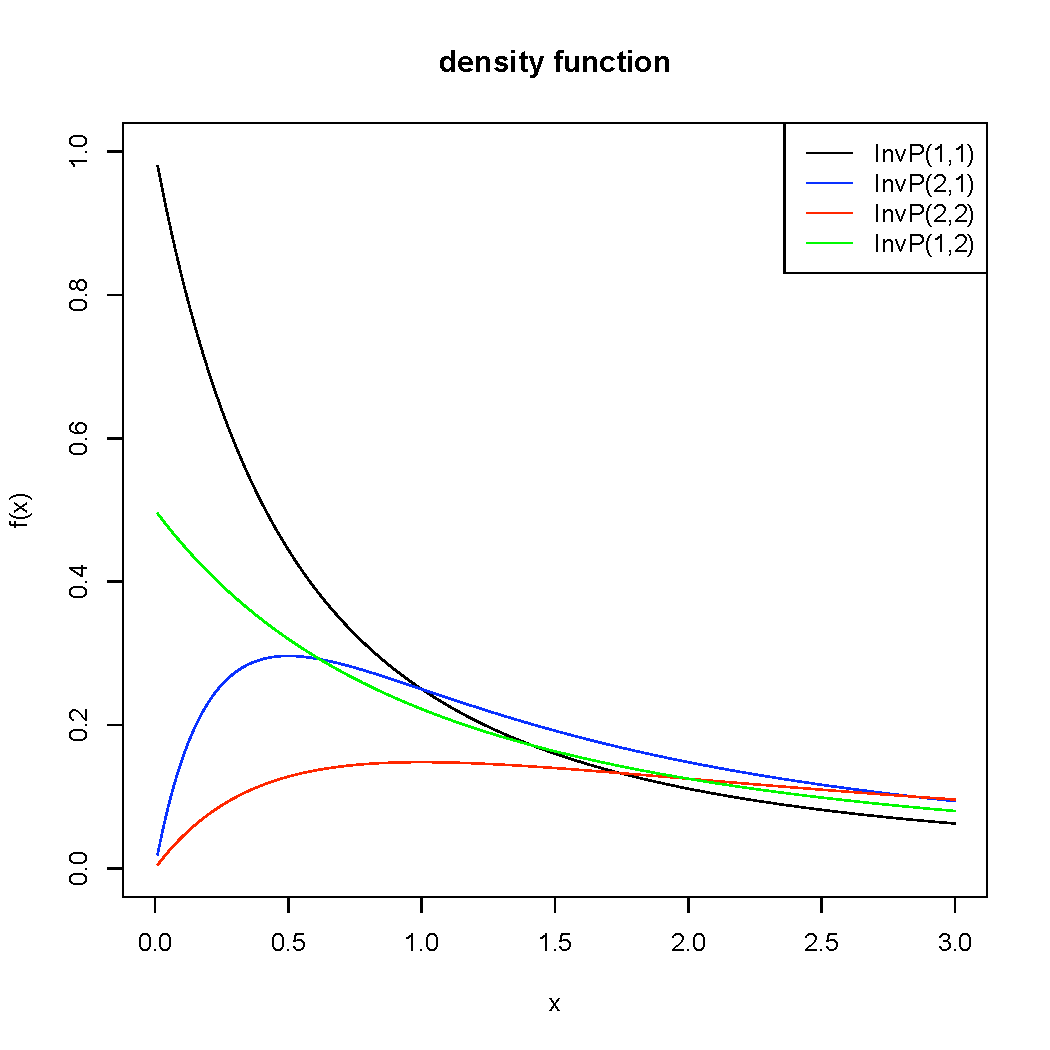
\includegraphics[width=0.48\textwidth]{img/invparetozoom}
  \end{center}
  \vspace{-20pt}  
  \caption{Density function for inverse Pareto distributions}
  \vspace{-20pt}  
\end{wrapfigure}
From the Feller-Pareto distribution, we get the inverse Pareto distribution with $\mu=0$,
$\delta_1=1$ and $\gamma=1$. Thus the density is
$$
f(x) =  \frac{1 }{ \beta(1, \delta_2)   }
\left(\frac{ \frac{x}{\sigma} }{ 1+\frac{x}{\sigma} } \right)^{\delta_2}  
\frac{ 1 }{ 1+\frac{x}{\sigma} } \frac{ 1 }{  \frac{x}{\sigma} },
$$
It can be rewritten as the density
$$
f(x) =  \frac{\tau\lambda x^{\tau-1}}{(x+\lambda)^{\tau+1}} 
$$
which implies the following distribution function
$$
F(x) = \left( \frac{x}{x+\lambda}\right)^\tau,
$$
for $x\geq 0$.
Let us note this is the distribution of $\frac{1}{X}$ when $X$ is Pareto II.

\subsection{Properties}
The expectation of the inverse Pareto distribution is $E(X) = \frac{\lambda\Gamma(\tau+1)}{\Gamma(\tau)}$, but the variance does not exist.

\subsection{Estimation}
NEED REFERENCE
\subsection{Random generation}
Simply inverse a Pareto II variable.

\subsection{Applications}
NEED REFERENCE

%%%%%%%%%%%%%%%%%%%%%%%%%%%%%%%%%%%%%%%%%%%%%%
\section{Generalized Pareto distribution}\label{GPD}
\subsection{Characterization}
\begin{wrapfigure}{r}{0.5\textwidth}
  \vspace{-50pt}
  \begin{center}
    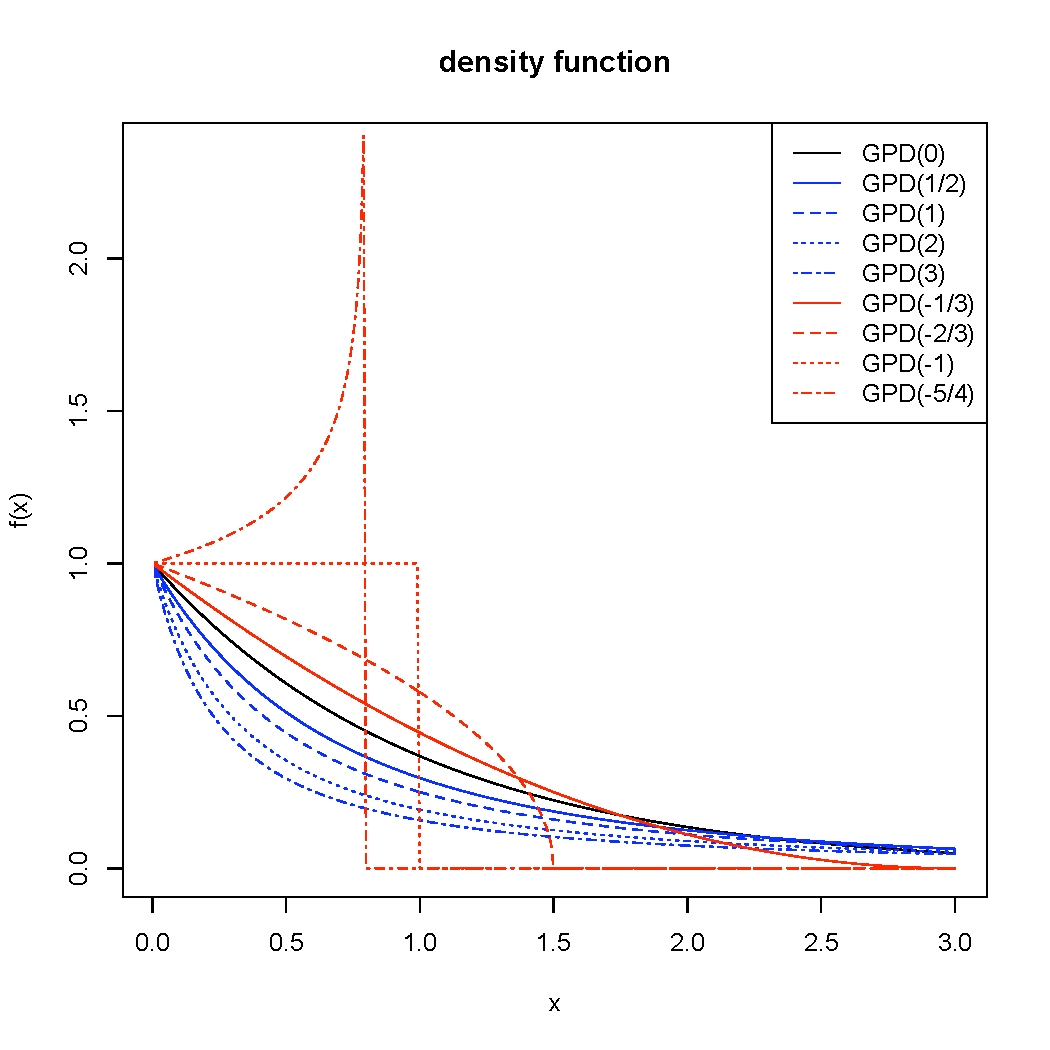
\includegraphics[width=0.48\textwidth]{img/gpdzoom}
  \end{center}
  \vspace{-20pt}  
  \caption{Density function for standard generalized Pareto distributions}
  \vspace{-20pt}  
\end{wrapfigure}

The generalized Pareto distribution was introduced in \cite{tve} in the context of extreme value theory.

We first define the standard generalized Pareto distribution by the following distribution function
$$
F(x) = \left\{
\begin{array}{ll}
1- \left(1+\xi x\right)^{-\frac{1}{\xi}} & \txtm{if} \xi \neq 0\\
1-e^{-x} & \txtm{if} \xi=0\\
\end{array}
\right. ,
$$
where $x\in\mbb R_+$ if $\xi\geq 0$ and $x\in\left[0, -\frac{1}{\xi}\right]$ otherwise. This distribution function is generally denoted by $G_\xi$.  

We can see the impact of the shape parameter $\xi$ on the figure on the right. The case where $\xi=0$ can be seen as a limiting case of $G_\xi$ when $\xi\rightarrow 0$.

To get the ``full'' generalized Pareto distribution, we introduce a scale $\beta$ and a location parameter $\mu$. We get
$$
F(x) = \left\{
\begin{array}{ll}
1- \left(1+\xi \frac{x-\nu}{\beta}\right)^{-\frac{1}{\xi}} & \txtm{if} \xi > 0\\
1-e^{-\frac{x-\nu}{\beta}} & \txtm{if} \xi=0\\
1- \left(1+\xi \frac{x-\nu}{\beta}\right)^{-\frac{1}{\xi}} & \txtm{if} \xi < 0\\
\end{array}
\right. ,
$$
where $x$ lies in $[\nu,+\infty[$, $[\nu,+\infty[$ and $\left[\nu, \nu-\frac{\beta}{\xi}\right]$ respectively. We denote it by $G_{\xi,\nu,\beta}(x)$ (which is simply $G_{\xi}(\frac{x-\nu}{\beta})$). Let us note when $\xi>0$, we have a Pareto II distribution, when $\xi=0$ a shifted exponential distribution and when $\xi<0$ a generalized beta I distribution.

From these expression, we can derive a density function for the generalized Pareto distribution
$$
f(x) = \left\{
\begin{array}{ll}
\frac{1}{\beta} \left(1+\xi \frac{x-\nu}{\beta}\right)^{-\frac{1}{\xi}-1} & \txtm{if} \xi > 0\\
\frac{1}{\beta} e^{-\frac{x-\nu}{\beta}} & \txtm{if} \xi=0\\
\frac{1}{\beta} \left(1-(-\xi) \frac{x-\nu}{\beta}\right)^{\frac{1}{-\xi}-1} & \txtm{if} \xi < 0\\
\end{array}
\right. ,
$$
for $x$ in the same supports as above. 


\subsection{Properties}
For a generalized Pareto distribution $G_{\xi,0,\beta}$, we have results on raw moments (for simplicity $\nu=0$). The expectation $E(X)$ is finite if and only if $\xi<1$. In this case we have
\begin{align*}
E\left(\left(1+ \frac{\xi}{\beta}X\right)^{-r}\right) = \frac{1}{1+\xi r}, \txtm{for} r>-\frac{1}{\xi}\\
E\left(\left(\log\left(1+ \frac{\xi}{\beta}X\right)\right)^k\right) = \xi^k k!, \txtm{for} k \in\mbb N\\
E\left(X \bar F(X)^r \right) = \frac{\beta}{(r+1-\xi)(r+1)}, \txtm{for} \frac{r+1}{|\xi|}>0\\
E\left(X^k\right) = \frac{\beta^k}{\xi^{k+1}} \frac{\Gamma(\xi^{-1}-k)}{\Gamma(1+\xi^{-1})} k!, \txtm{for} \xi <\frac{1}{k},
\end{align*}
see \cite{tve} for details.

If $X$ follows a generalized Pareto distribution $GPD(\xi,0,\beta)$, then the treshold excess random variable $X-u| X>u$ still follows a generalized Pareto distribution $GPD(\xi,0,\beta+\xi u)$. Let $F_u$ be the distribution function of $X-u| X>u$.
We have $F$ is in the maximum domain of attraction $H_\xi$ if and only if 
$$
\underset{u\rightarrow x_f}{\lim} \underset{0<x<x_f-u}{\sup}  \left|F_u(x) - G_{\xi,0,\beta(u)}(x)  \right| = 0,
$$
where $\beta$ is a positive function. This makes the link between the generalized Pareto distribution and the generalized extreme value distribution.


\subsection{Estimation}
In this sub-section, we assume $\nu=0$.

\subsubsection{Peak Over a Treshold}
We briefly present the Peak Over a Treshold (POT) method to fit the generalized Pareto distribution. Let $(X_i)_{1\leq i\leq n}$ an i.i.d. sample whose distribution function belongs to a maximum domain of attraction  $H_\xi$. For a deterministic treshold $u>0$, we define the number of exceedances by
$$
N_u %=\card \Delta_u
= \card(1\leq i\leq n, X_i>u),
$$
with the corresponding excesses $(Y_i)_{1\leq i \leq N_u}$. We want to fit the excess distribution function $F_u$ with the GPD distribution function $G_{\xi,0,\beta(u)}$.

First we can use the linearity of the mean excess function
$$
E(X-u | X>u) = \frac{\beta+\xi u}{1-\xi},
$$
for a given $u$. This can be estimated by the empirical mean of the sample $(Y_i)_{1\leq i \leq N_u}$. \cite{tve} warn us about the difficulty of chosing $u$, since they are many $u$ for wich the plot of 
$(u, \bar Y_{N_u})$.

Once we find the treshold $u$, we can use conditional likelihood estimation on sample $(Y_i)_{1\leq i \leq N_u}$. Let $\tau$ be $ -\xi/\beta$. However we can also use a linear regression to fit the shape and the scale parameter.


\subsubsection{Maximum likelihood estimation}
Maximum likelihood estimators of $\xi$ and $\beta$ are solutions of the system
$$
\left\{
\begin{array}{l}
 \left(\frac{1}{\xi}+1\right)\sum\limits_{i=1}^n \frac{\xi X_i}{\beta^2+\beta \xi X_i} = \frac{n}{\beta}\\
 \frac{1}{\xi^2}\sum\limits_{i=1}^n\log\left(1+\frac{\xi}{\beta}X_i\right) = (\frac{1}{\xi}+1)\sum\limits_{i=1}^n\frac{X_i}{\beta+\xi X_i}
 \end{array}
 \right. ,
$$
but the system may be instable for $\xi\leq-1/2$. When $\xi>1/2$, we have some asymptotical properties of maximum likelihood estimators $\hat \xi$ and $\hat \beta$:
$$
\sqrt{n}\left(\hat\xi -\xi, \frac{\hat\beta}{\beta}-1\right) \stackrel{\mcal L}{\longrightarrow} \mcal N(0,M^{-1}),
$$
where the variance/covariance matrix for the bivariate normal distribution is
$$
M^{-1} = (1+\xi)\left(
\begin{array}{cc}
1+\xi & 1\\
1 & 2
\end{array}
\right) .
$$
Let us note that if we estimate a $\xi$ as zero, then we can try to fit a shifted exponential distribution.

\subsubsection{Method of moments}
From the properties, we know the theoretical expression of $E(X)$ and $E\left(X \bar F(X) \right)$. From wich we get the relation 
$$
\beta = \frac{2E(X)E\left(X \bar F(X) \right)}{E(X)-2E\left(X \bar F(X) \right)} \txtm{and} \xi = 2-\frac{E(X)}{E(X)-2E\left(X \bar F(X) \right)}.
$$
We simply replace $E(X)$ and $E\left(X \bar F(X) \right)$ by the empirical estimators.

\subsection{Random generation}
We have an explicit expression for the quantile function
$$
F^{-1}(u) = \left\{
\begin{array}{ll}
\nu+\frac{\sigma}{\xi}((1-u)^{-\xi}-1) & \txtm{if} \xi \neq 0\\
\nu-\sigma\log(1-u) & \txtm{if} \xi=0\\
\end{array}
\right.,
$$
thus we can use the inversion function method to generate GPD variables.

\subsection{Applications}
The main application of the generalized Pareto distribution is the extreme value theory, since there exists a link between the generalized Pareto distribution and the generalized extreme value distribution. Typical applications are modeling flood in hydrology, natural disaster in insurance and asset returns in finance.

%%%%%%%%%%%%%%%%%%%%%%%%%%%%%%%%%%%%%%%%%%%%%%
\section{Burr distribution}
\subsection{Characterization}
\begin{wrapfigure}{r}{0.5\textwidth}
  \vspace{-40pt}
  \begin{center}
    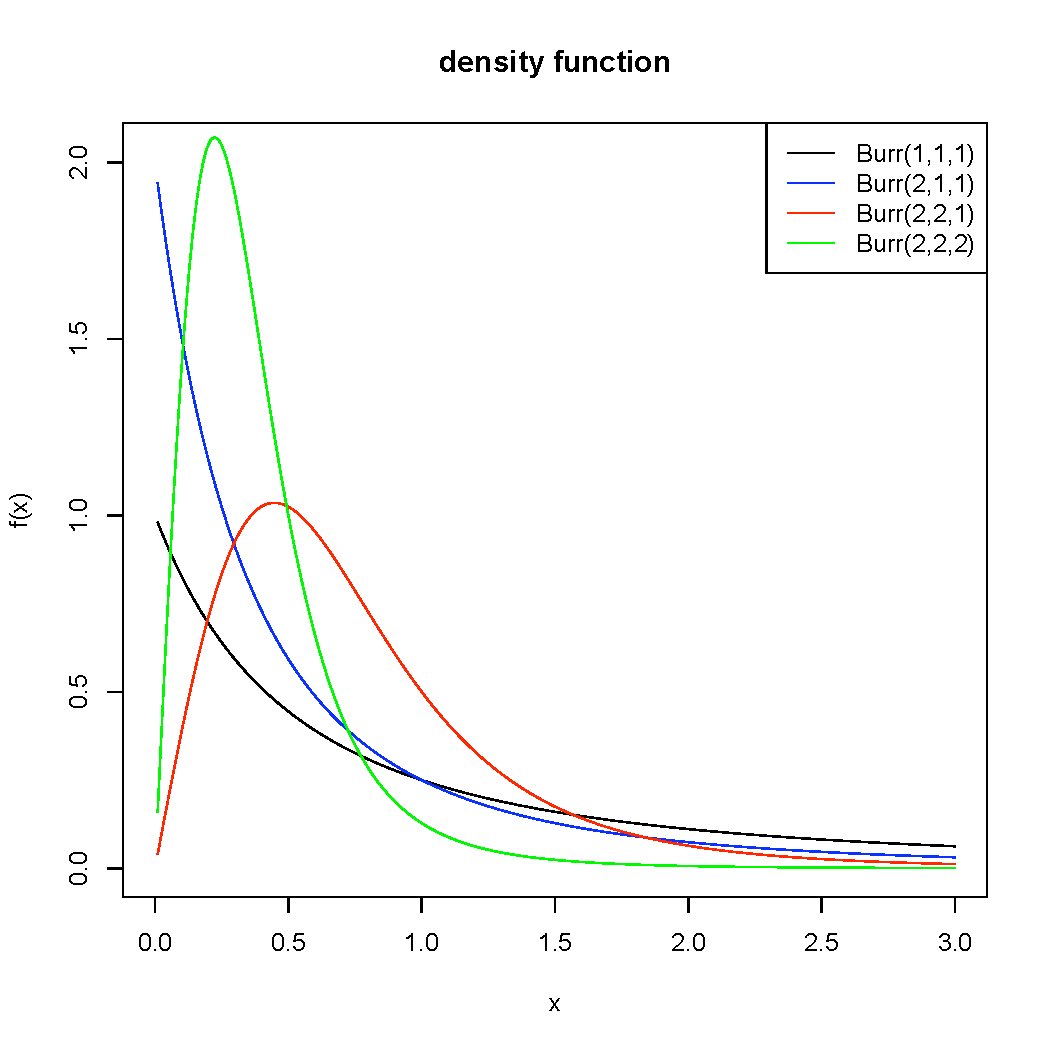
\includegraphics[width=0.48\textwidth]{img/burrzoom}
  \end{center}
  \vspace{-20pt}  
  \caption{Density function for Burr distributions}
  \vspace{-20pt}  
\end{wrapfigure}
The Burr distribution is defined by the following density
$$
f(x) =\frac{\alpha\tau}{\lambda} \frac{  (x/\lambda)^{\tau-1}}{(1+(x/\lambda)^\tau)^{\alpha+1}}
$$
where $x\geq0$, $\lambda$ the scale parameter and $\alpha,\tau>0$ the shape parameters. 
Its distribution function is given by
$$
F(x) = 1-\left(\frac{\lambda^\tau}{\lambda^\tau+x^\tau}\right)^{\alpha},
$$
for $x\geq 0$.
In a slightly different rewritten form, we recognise the Pareto IV distribution
$$
\bar F(x) = \left(1+\left(\frac{x}{\lambda}\right)^\tau\right)^{-\alpha},
$$
with a zero location parameter.

\subsection{Properties}
The raw moment of the Burr distribution is given by 
$$
E(X^r) = \lambda^r\frac{\Gamma(1+\frac{r}{\tau})\Gamma(\alpha-\frac{r}{\tau})}{\Gamma(\alpha)},
$$
hence the expectation and the variance are 
$$
E(X) = \lambda\frac{\Gamma(1+\frac{1}{\tau})\Gamma(\alpha-\frac{1}{\tau})}{\Gamma(\alpha)} \txtm{and}
Var(X) = \lambda^2\frac{\Gamma(1+\frac{2}{\tau})\Gamma(\alpha-\frac{2}{\tau})}{\Gamma(\alpha)} -\left(\lambda\frac{\Gamma(1+\frac{1}{\tau})\Gamma(\alpha-\frac{1}{\tau})}{\Gamma(\alpha)}\right)^2.
$$

\subsection{Estimation}
Maximum likelihood estimators are solution of the system
$$
\left\{
\begin{array}{l}
\frac{n}{\alpha}=\sum\limits_{i=1}^n\log \left(1+ \left(\frac{X_i}{\lambda}\right)^\tau\right)\\
\frac{n}{\tau}=-\sum\limits_{i=1}^n\log \left(\frac{X_i}{\lambda}\right)
+\tau\frac{\alpha+1}{\lambda}\sum\limits_{i=1}^n \log \left(\frac{X_i}{\lambda}\right) \frac{X_i^\tau}{\lambda^\tau+X_i^\tau}\\
\frac{n}{\lambda} = -\frac{\tau-1}{\lambda}\sum\limits_{i=1}^n\frac{1}{X_i}
+\tau\frac{\alpha+1}{\lambda}\sum\limits_{i=1}^n\frac{1}{\lambda^\tau+X_i^\tau}
\end{array}
\right. ,
$$
which can be solved numerically.

\subsection{Random generation}
From the quantile function $F^{-1}(u) = \lambda((1-u)^{\frac{1}{\alpha}} -1 )^{\frac{1}{\tau}}$, it is easy to generate Burr random variate with $\lambda(U^{\frac{1}{\alpha}} -1 )^{\frac{1}{\tau}}$ where $U$ is a uniform variable.

\subsection{Applications}
NEED REFERENCE

%%%%%%%%%%%%%%%%%%%%%%%%%%%%%%%%%%%%%%%%%%%%%%
\newpage
\section{Inverse Burr distribution}
\subsection{Characterization}
\begin{wrapfigure}{r}{0.5\textwidth}
  \vspace{-40pt}
  \begin{center}
    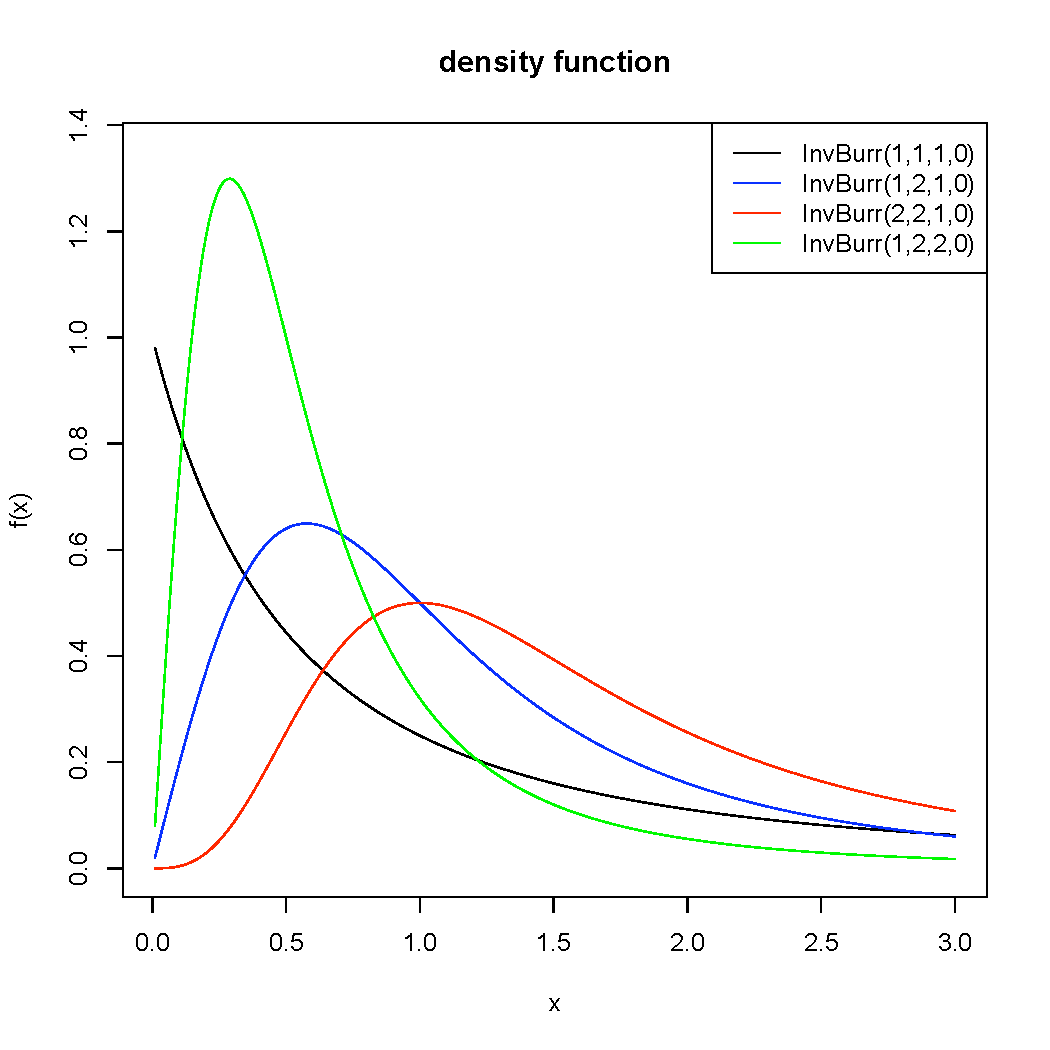
\includegraphics[width=0.48\textwidth]{img/invburrzoom}
  \end{center}
  \vspace{-20pt}  
  \caption{Density function for inverse Burr distributions}
  \vspace{-20pt}  
\end{wrapfigure}
The inverse Burr distribution (also called the Dagum distribution) is a special case of the Feller Pareto distribution $\mcal F\mcal P$ with $\delta_2=1$. That is to say the density is given by
$$
f(x) = \frac{\alpha\gamma}{\sigma} \frac{\left(\frac{x-\mu}{\sigma}\right)^{\alpha\gamma-1}}{\left(1+\left(\frac{x-\mu}{\sigma}\right)^{\alpha}\right)^{\gamma+1}},
$$
where $x\leq \mu$, $\mu$ the location parameter, $\sigma $ the scale parameter and $\alpha,\gamma$ the shape parameters. \cite{klugman} defines the inverse Burr distribution with $\mu=0$, 
%$$
%f(x) = \frac{\alpha\gamma}{\beta} \frac{\left(\frac{x}{\beta}\right)^{\alpha\gamma-1}}{\left(1+\left(\frac{x}{\beta}\right)^{\alpha}\right)^{\gamma+1}},
%$$
since this book deals with insurance loss distributions. In this expression, it is not so obvious that this is the inverse Burr distribution and not the Burr distribution. But the density can be rewritten as
$$
f(x) = \frac{\alpha\gamma}{\sigma} \frac{\left(\frac{\sigma}{x-\mu}\right)^{\alpha+1}}{\left(\left(\frac{\sigma}{x-\mu}\right)^{\alpha}+1\right)^{\gamma+1}},
$$
From this, the distribution function can be derived to 
$$
F(x) =\left(\frac{1}{\left(\frac{\sigma}{x-\mu}\right)^\alpha+1}\right)^{\gamma},
$$
for $x\geq \mu$. Here it is also clearer that this is the inverse Burr distribution since we notice the survival function of the Burr distribution taken in $\frac{1}{x}$. We denotes the inverse Burr distribution by $\mcal I\mcal B(\gamma,\alpha,\beta,\mu)$.

\subsection{Properties}
The raw moments of the inverse Burr distribution are given by
$$
E(X^r) = \sigma^r\frac{\Gamma(\gamma+\frac{r}{\alpha})\Gamma(1-\frac{r}{\alpha})}{\Gamma(\gamma)},
$$
when $\mu=0$ and $\alpha>r$. Thus the expectation and the variance are
$$
E(X) = \mu+\sigma\frac{\Gamma(\gamma+\frac{1}{\alpha})\Gamma(1-\frac{1}{\alpha})}{\Gamma(\gamma)}
$$
and 
$$
Var(X) = \sigma^2\frac{\Gamma(\gamma+\frac{2}{\alpha})\Gamma(1-\frac{2}{\alpha})}{\Gamma(\gamma)}-\sigma^2\frac{\Gamma^2(\gamma+\frac{1}{\alpha})\Gamma^2(1-\frac{1}{\alpha})}{\Gamma^2(\gamma)}
$$

Furthermore, we have the following special cases
\begin{itemize}
\item with $\gamma=\alpha$, we get the inverse paralogistic distribution,
\item with $\gamma=1$, we have the log logistic distribution,
\item with $\alpha=1$, this is the inverse Pareto distribution.
\end{itemize}

\subsection{Estimation}
The maximum likelihood estimator of $\mu$ is simply $\hat\mu=X_{1:n}$ for a sample $(X_i)_i$, then working on the transformed sample $Y_i=X_i-\hat\mu$, other maximum likelihood estimators are solutions of the system
$$
\left\{
\begin{array}{l}
\frac{n}{\gamma}=\sum\limits_{i=1}^n\log \left(1+ \left(\frac{\lambda}{Y_i}\right)^\alpha\right)\\
\frac{n}{\alpha}=-\sum\limits_{i=1}^n\log \left(\frac{\sigma}{Y_i}\right)
+(\gamma+1)\sum\limits_{i=1}^n  \log \left(\frac{\sigma}{Y_i}\right) \frac{\sigma^\alpha}{Y_i^\alpha+\sigma^\alpha}\\
\frac{n}{\sigma} = (\alpha+1)\sum\limits_{i=1}^n\frac{1}{Y_i+\sigma}
-\alpha\frac{\gamma+1}{\sigma}\sum\limits_{i=1}^n\frac{\sigma^\alpha}{Y_i^\alpha+\sigma^\alpha}
\end{array}
\right. ,
$$

\subsection{Random generation}
Since the quantile function is $F^{-1}(u) = \mu+\sigma^{-1}(u^{-\frac{1}{\gamma}}-1)^{-\frac{1}{\alpha}}$, we can use the inverse function method.

\subsection{Applications}
NEED REFERENCE

%%%%%%%%%%%%%%%%%%%%%%%%%%%%%%%%%%%%%%%%%%%%%%
\section{Beta type II distribution}
\subsection{Characterization}
There are many ways to characterize the beta type II distribution. First we can say it is the distribution of
$\frac{X}{1-X}$ when $X$ is beta I distributed. But this is also the distribution of the ratio $\frac{U}{V}$ when $U$ and $V$ are gamma distributed ($\mcal G(a,1)$ and $\mcal G(b,1)$ resp.).
The distribution function of the beta of the second distribution is given by
$$
F(x) = \frac{\beta(a,b,\frac{x}{1+x})}{\beta(a, b)},
$$
for $x\leq 0$. The main difference with the beta I distribution is that the beta II distribution takes values in $\mbb R_+$ and not $[0,1]$.

The density can be expressed as
$$
f(x) = \frac{x^{a-1}}{\beta(a, b) (1+x)^{a + b}},
$$
for $x\leq 0$. It is easier to see the transformation $\frac{x}{1-x}$ if we rewrite the density as
$$
f(x) = \left(\frac{x}{1+x}\right)^{a-1}\left(1-\frac{x}{1+x}\right)^{b-1}\frac{1}{\beta(a,b)(1+x)^2}.
$$
As already mentioned above, this is a special case of the Feller-Pareto distribution.
\subsection{Properties}
The expectation and the variance of the beta II are given by $E(X) = \frac{a}{b-1}$ and $Var(X) = \frac{a(a+b-1)}{(b-1)^2(b-2)}$ when $b>1$ and $b>2$.
Raw moments are expressed as follows 
$$
E(X^r) =  \frac{\Gamma(a+r)
\Gamma(b-r)}{\Gamma(a)\Gamma(b)},
$$
for $b>r$.

\subsection{Estimation}
Maximum likelihood estimators for $a$ and $b$ verify the system
$$
\left\{
\begin{array}{l}
\psi(a)-\psi(a+b) = \frac{1}{n}\sum\limits_{i=1}^n(\log(1+X_i)-\log(X_i))\\
\psi(b)-\psi(a+b) = \frac{1}{n}\sum\limits_{i=1}^n\log(1+X_i)\\
\end{array}
\right. ,
$$
where $\psi$ denotes the digamma function. We may also use the moment based estimators given by
$$
\tilde b = 2 + \frac{\bar X_n(\bar X_n+1)}{S_n^2} \txtm{and} \tilde a=(\tilde b-1)\bar X_n,
$$
which have the drawback that $\tilde b$ is always greater than 2.


\subsection{Random generation}
We can simply use the construction of the beta II, i.e. the ratio of $\frac{X}{1-X}$ when $X$ is beta I distributed. However we may also use the ratio of two gamma variables.

\subsection{Applications}
NEED REFERENCE

